%!TEX root = main.tex

\toclesssection{Introduction and Motivation}

\begin{frame}{Introduction and Motivation}{The Simulation of Dynamic Systems}
  \begin{columns}
    \begin{column}[c]{0.6\textwidth}
      \uncover<1->{%
        \hi{\large Why do we need simulation?} \\
        It is used to \dots \\
        \begin{itemize}\small
          \item[\raisebox{-1pt}{\scalebox{0.8}{\faCogs}}] \emph{predict} the behavior
          \item[\raisebox{-1pt}{\scalebox{0.8}{\faConnectdevelop}}] \emph{design} and \emph{optimize}
          \item[\raisebox{-1pt}{\scalebox{0.8}{\faHourglassStart}}] accelerate development and testing
          \item[\raisebox{-1pt}{\scalebox{0.8}{\faCarCrash}}] risk-free testing environment
          \item[\raisebox{-1pt}{\scalebox{0.8}{\faDollarSign}}] \emph{reduce} development costs
        \end{itemize}
      }
      \vspace{0.5em}
      \uncover<2->{%
        \hi{\large Simulations' \textbf{complexity} is increasing!} \\
        Higher \textbf{fidelity}, more \textbf{complexity}, more \dots \\
        \begin{itemize}\small
          \item[\raisebox{-1pt}{\scalebox{0.8}{\faCog}}] components \\
          \item[\raisebox{-1pt}{\scalebox{0.8}{\faCompress}}] interactions \\
          \item[\raisebox{-1pt}{\scalebox{0.8}{\faDesktop}}] computational resources \\
          \item[\raisebox{-1pt}{\scalebox{0.8}{\faHourglassEnd}}] computation time
        \end{itemize}
      }
      \end{column}
    \begin{column}[c]{0.4\textwidth}
      \centering
      \uncover<3->{\hic{\large A ``random'' example}}
      \only<-2>{
        \hic{\Huge{\textbf{?}} \\[0.5em]
        \normalsize{\dots something we've never seen before!}}
      }
      \only<3->{\includegraphics[
          width=0.52\textwidth, trim={0cm 0cm 4.65cm 0cm}, clip
        ]{figures/vehicle_modules.eps}
      }
    \end{column}
  \end{columns}
\end{frame}

\subsection{Dynamic Systems as a Collection of Subsystems}

\begin{frame}{Introduction and Motivation}{Dynamic Systems as a Collection of Subsystems}
  \begin{columns}
    \begin{column}[c]{0.6\textwidth}
      \begin{itemize}
        \item<1-> Complex systems are divided into \textbf{subsystems} \dots \\
        \begin{small}
          \quad\, \begin{tabular}{ccc}
            \raisebox{-1pt}{\scalebox{0.8}{\textcolor{fg_sl_color}{\faCogs}}} mechanical &
            \raisebox{-1pt}{\scalebox{0.8}{\textcolor{fg_sl_color}{\faBolt}}} electrical &
            \raisebox{-1pt}{\scalebox{0.8}{\textcolor{fg_sl_color}{\faFire}}} thermal \\
            \raisebox{-1pt}{\scalebox{0.8}{\textcolor{fg_sl_color}{\faOilCan}}} hydraulic &
            \raisebox{-1pt}{\scalebox{0.8}{\textcolor{fg_sl_color}{\faWaveSquare}}} control & \dots
          \end{tabular}
        \end{small}
        \item<3-> Subsystems are described by \textbf{equations} \dots \\
        \begin{small}
          \qquad \emph{algebraic} \\
          \qquad ordinary \emph{differential} \\
          \qquad \emph{differential-algebraic} \\
          \qquad other types
        \end{small}
        \item<4-> The \textbf{challenges} are \dots \hic{\normalsize Speed \qquad Accuracy \qquad Efficiency}
      \end{itemize}
    \end{column}
    \begin{column}[c]{0.4\textwidth}
      \centering
      \hic{\large A ``random'' example}
      \only<1>{\includegraphics[
          width=0.52\textwidth, trim={0cm 0cm 4.65cm 0cm}, clip
        ]{figures/vehicle_modules.eps}}
      \only<2->{
        \includegraphics[width=\textwidth]{figures/vehicle_modules.eps}}
    \end{column}
  \end{columns}
\end{frame}

\subsection{Solution Approaches}

\begin{frame}{Introduction and Motivation}{Solution Approaches}
  \begin{columns}
    \begin{column}[c]{0.45\textwidth}
      The \textbf{solution} of these equations can be \dots \\
      \begin{itemize}[<+->]
        \item \textbf{Analytical} \\
        \begin{small}
          \qquad \textcolor{mycolor2!95!black}{deep understanding of the problem} \\
          \qquad \textcolor{mycolor2!95!black}{rare and difficult to achieve} \\
          \qquad \textcolor{mycolor5!95!black}{low computational resources}
        \end{small}
        \item \textbf{Numerical} \\
        \begin{small}
          \qquad \textcolor{mycolor5!95!black}{well-established and widely used} \\
          \qquad \textcolor{mycolor3!95!black}{not always the applicable} \\
          \qquad \textcolor{mycolor2!95!black}{high computational resources}
        \end{small}
        \item \textbf{Mixed analytical/numerical} \\
        \begin{small}
          \qquad \textcolor{mycolor3!95!black}{\emph{ad hoc}, for specific cases} \\
          \qquad \textcolor{mycolor3!95!black}{limited applicability} \\
          \qquad \textcolor{mycolor3!95!black}{reduced computational resources}
        \end{small}
      \end{itemize}
      \uncover{\hic{\normalsize
        These examples are special cases! \\
        \emph{What about more general systems?}
      }}
    \end{column}
    \begin{column}[c]{0.6\textwidth}
      \centering
      \small
      \vspace{-2.0em}
      \begin{tabular}{>{\centering\arraybackslash} m{3.75cm} >{\centering\arraybackslash} m{3.75cm}}
        \visible<1->{\includegraphics[width=0.4\textwidth]{figures/fade_overview.png} &
        \vspace{-2.0em}$\begin{array}{c}
          \text{\hi{Direct stiffness method (A4)}} \\[0.25em]
          \begin{bmatrix}
            \mathbf{K}_{ff} & \mathbf{K}_{fs} \\
            \mathbf{K}_{sf} & \mathbf{K}_{ss}
          \end{bmatrix} \begin{bmatrix}
            \mathbf{d}_{f} \\
            \mathbf{d}_{s}
          \end{bmatrix} = \begin{bmatrix}
            \mathbf{f}_{f} \\
            \mathbf{f}_{s}
          \end{bmatrix}
        \end{array}$} \\
        \visible<2->{\vspace{-3.0em}$\msmall{\begin{array}{c}
          \text{\hi{Tire-road interaction (A1-2)}} \\[0.25em]
          \mathbf{P} = \frac{1}{V} \int\nolimits_\mathcal{V} \text{proj}(\mathbf{x}, \partial\mathcal{G}) \, \text{d}\mathcal{\mathbf{x}} \\[0.1em]
          \mathbf{\hat{n}} = \int\nolimits_\mathcal{V} \mathbf{d}(\mathbf{x},\mathbf{h}_y) \, \text{d}\mathcal{\mathbf{x}}
        \end{array}}$ &
        \includegraphics[width=0.4\textwidth]{figures/enve_intersection.png}} \\
        \visible<3->{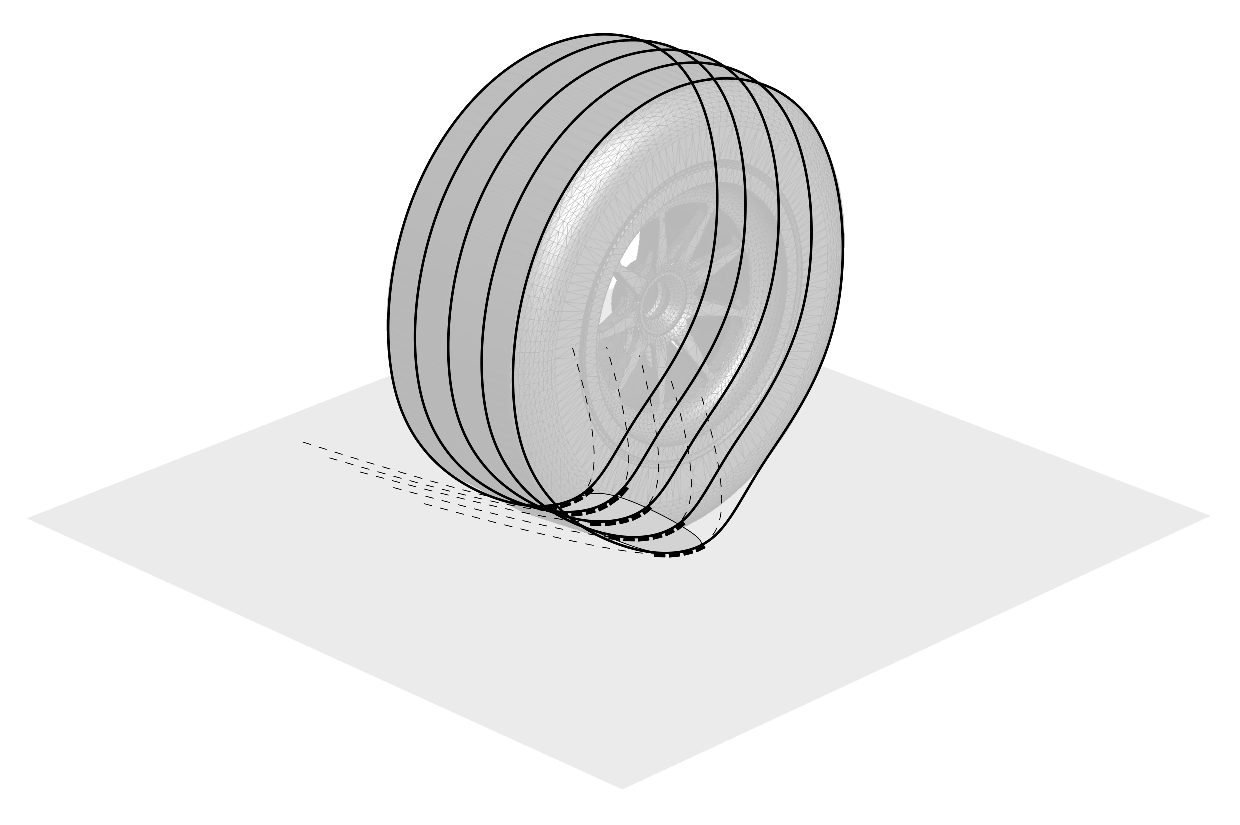
\includegraphics[
          width=0.35\textwidth, trim={4.5cm 3.5cm 4.5cm 0cm}, clip
          ]{figures/brush_model_simplified.eps} &
        \vspace{-3.0em}$\msmall{\begin{array}{c}
          \text{\hi{Tire model (A3)}} \\[0.25em]
            \mathbf{F}(F_z, \sigma_x, \sigma_y, \varphi, \gamma, p, T, t) \\[0.1em]
            \mathbf{M}(F_z, \sigma_x, \sigma_y, \varphi, \gamma, p, T, t)
        \end{array}}$}
      \end{tabular}
    \end{column}
  \end{columns}
\end{frame}

\subsection{Dynamic Systems Described by \acsp{ODE} and \acsp{DAE}}

\begin{frame}{Introduction and Motivation}{Dynamic Systems Described by \acsp{ODE} and \acsp{DAE}}
  \begin{itemize}[<+->]
    \item Typically, \textbf{dynamic systems} are described by \dots \\
      \vspace{0.5em}
      \setlength{\tabcolsep}{3.5em}
      \centering{\small\begin{tabular}{cc}
          \hi{\acsp{ODE}}                                               & \hi{\acsp{DAE}} \\
          \textcolor{mycolor5!95!black}{Easy to initialize}            & \textcolor{mycolor2!95!black}{Hard to initialize} \\
          \textcolor{mycolor5!95!black}{Strong theoretical foundation} & \textcolor{mycolor3!95!black}{Complex theoretical foundation} \\
          \textcolor{mycolor5!95!black}{Efficient numerical methods}   & \textcolor{mycolor3!95!black}{Require \emph{ad hoc} numerical methods} \\
          \textcolor{mycolor2!95!black}{Some models do not fit}        & \textcolor{mycolor5!95!black}{State-of-the-art in modeling} \\
      \end{tabular}}
    \vspace{0.25em}
    \item \acsp{ODE} have a \textbf{complete} theoretical foundation, \acsp{DAE} do not
    \item Existing tools for \acsp{DAE} are not as \textbf{mature} and \textbf{efficient} as \acsp{ODE} tools
    \item From an engineering perspective, this is a \textbf{problem} (\textcolor{fg_sl_color}{\faHourglassHalf\,\faDollarSign\,\faCarCrash\,\faSadTear})
    %\begin{small}
    %\qquad high level of applicability, \emph{but not very widely used!} \\
    %\qquad effective in the solution of \acsp{ODE}, \emph{but what about \acsp{DAE}?}
    %\end{small}
    %\item<4-> Existing tools are mainly based on \textbf{numerical} or \textbf{structural analysis} techniques
  \end{itemize}
  \uncover<5->{
    \centering
    \vspace{0.5em}
    Therefore, the question is \dots \\[-1.0em]
    \hic{\large How can we improve the state-of-the-art in the solution of \acsp{DAE}?}
  }
  %\hic{Exploit symbolic computation in the solution of \acsp{DAE}!}
\end{frame}

% That's all Folks!
